% Transcrito de Documento_Visao_MotivaFit_Completo_e_Detalhado.pdf
\clearpage
\section{VISÃO GERAL DO PROJETO}

O desenvolvimento do projeto é conduzido sob uma abordagem ágil e iterativa, unindo a estrutura de gestão do Scrum (focada em Sprints curtas e entregas contínuas de valor) às práticas de engenharia do eXtreme Programming (XP) [4, 5]. O trabalho é sustentado por Pair Programming, revisões de código e uma esteira automatizada de Integração Contínua (CI) para garantir entregas seguras e alinhadas às necessidades do usuário.

\subsection{CICLO DE VIDA DO PROJETO}

O projeto adotará metodologias ágeis baseadas no framework Scrum, com iterações (Sprints) de uma semana. Essa abordagem visa entregas incrementais focadas em valor, permitindo a validação contínua de funcionalidades motivacionais com os usuários.

A Figura~\ref{fig:ciclo_de_vida} apresenta a sequência adotada: o Product Backlog reúne as necessidades do produto; na Sprint Planning, a equipe seleciona os itens e define o Sprint Backlog. A execução ocorre em uma Sprint de uma semana. Ao final, a Review avalia a entrega com os interessados e a Retrospectiva identifica melhorias no processo. O incremento representa a funcionalidade concluída que amplia o produto. Embora a imagem apresente uma sequência linear, o processo é repetido a cada Sprint, com atualização do backlog e incorporação das melhorias identificadas [5].

\begin{figure}[htbp]
\centering
\caption{Ciclo de vida do projeto}
\label{fig:ciclo_de_vida}
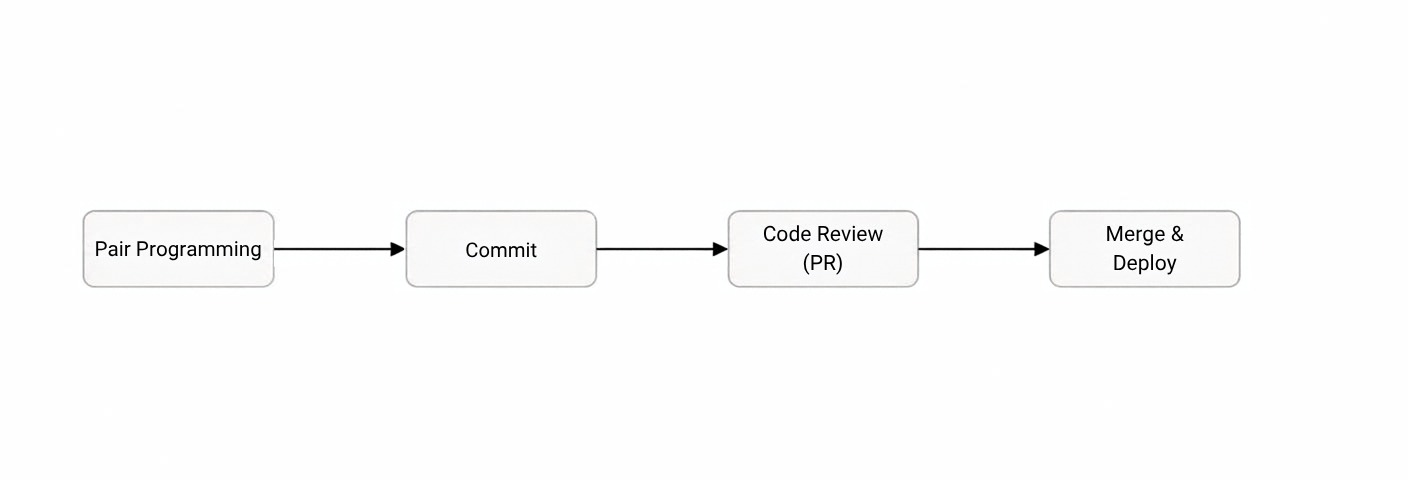
\includegraphics[width=\linewidth,keepaspectratio]{imgs/ciclo_de_vida.jpeg}
\par\smallskip
{\fontedez Fonte: elaborado pelos autores (2026), com base no Guia do Scrum [5].}
\end{figure}
\FloatBarrier

\begingroup
\small
\setlength{\tabcolsep}{3pt}
\renewcommand{\arraystretch}{1.2}
\begin{longtable}{|>{\raggedright\arraybackslash}p{\dimexpr 0.220\linewidth-2\tabcolsep-1.5\arrayrulewidth\relax}|>{\raggedright\arraybackslash}p{\dimexpr 0.780\linewidth-2\tabcolsep-1.5\arrayrulewidth\relax}|}
\hline
\textbf{Aspecto} & \textbf{Definição} \\ \hline
\endfirsthead
\textbf{Aspecto} & \textbf{Definição} \\ \hline
\endhead
Metodologia & Desenvolvimento Ágil. \\ \hline
Processo & Scrum. \\ \hline
Procedimentos & Sprint Planning, Code Review, Pair Programming, Integração Contínua, Refinamento do Backlog e Sprint Reviews. \\ \hline
Métodos & UML (Unified Modeling Language, linguagem de modelagem unificada), User Stories, Planning Poker, MoSCoW, Análise de Pontos de Função. \\ \hline
Ferramentas & Git, GitHub, Figma, VS Code, IntelliJ, Docker, Postman, Maven. \\ \hline
\end{longtable}
\noindent{\fontedez Fonte: elaborado pelos autores (2026).}
\endgroup

\subsection{ORGANIZAÇÃO DO PROJETO}

\begingroup
\small
\setlength{\tabcolsep}{4pt}
\renewcommand{\arraystretch}{1.2}
\begin{longtable}{|>{\raggedright\arraybackslash}p{\dimexpr 0.270\linewidth-2\tabcolsep-1.5\arrayrulewidth\relax}|>{\raggedright\arraybackslash}p{\dimexpr 0.430\linewidth-2\tabcolsep-1.5\arrayrulewidth\relax}|>{\raggedright\arraybackslash}p{\dimexpr 0.300\linewidth-2\tabcolsep-1.5\arrayrulewidth\relax}|}
\caption{Papéis e responsabilidades}\\
\hline
\textbf{Papel} & \textbf{Atribuições} & \textbf{Responsável} \\ \hline
\endfirsthead
\textbf{Papel} & \textbf{Atribuições} & \textbf{Responsável} \\ \hline
\endhead
Desenvolvedor Backend & Codificar o produto, codificar testes unitários, realizar refatoração. Estruturar a lógica de funcionamento do app. & Matheus Estevam, Luis, Lucas \\ \hline
Desenvolvedor Frontend & Codificar o produto, codificar testes unitários, realizar refatoração. Desenvolver a interface de usuário do app. & Rafael Laube, Mateus Fernandes \\ \hline
Documentação & Confecção dos documentos para entrega. & Bruno \\ \hline
Dono do Produto & Atualizar o escopo do produto, organizar o escopo das sprints, validar as entregas. & Monitor Daniel \\ \hline
Analista de Qualidade & Garantir a qualidade do produto, garantir o cumprimento do conceito de pronto, realizar inspeções de código. & Bernardo \\ \hline
Cliente & Validar negócio e expectativas. & Ricardo Ajax \\ \hline
\end{longtable}
\noindent{\fontedez Fonte: elaborado pelos autores (2026).}
\endgroup

\subsubsection{ANÁLISE CAUSAL}

O diagrama de Ishikawa organiza possíveis causas de um problema em categorias, relacionando-as ao efeito analisado [12]. Na Figura~\ref{fig:ishikawa}, o efeito é o abandono de atividades físicas e a desmotivação. Os ramos apresentam falta de planejamento, ausência de engajamento e falta de percepção de evolução, com suas causas específicas e os requisitos propostos para enfrentá-las:

\begin{itemize}
\item Falta de planejamento: desorganização de rotinas e divisões musculares inadequadas. Origina a necessidade de cadastro de treino (RF-03).
\item Ausência de engajamento: treinos monótonos, tédio e falta de incentivo social. Origina as conquistas (RF-22) e a submissão de desafios (RF-18).
\item Falta de percepção de evolução: dificuldade em perceber resultados rápidos. Origina o acompanhamento de métricas (RF-12).
\end{itemize}

\begin{figure}[htbp]
\centering
\caption{Diagrama de Ishikawa}
\label{fig:ishikawa}
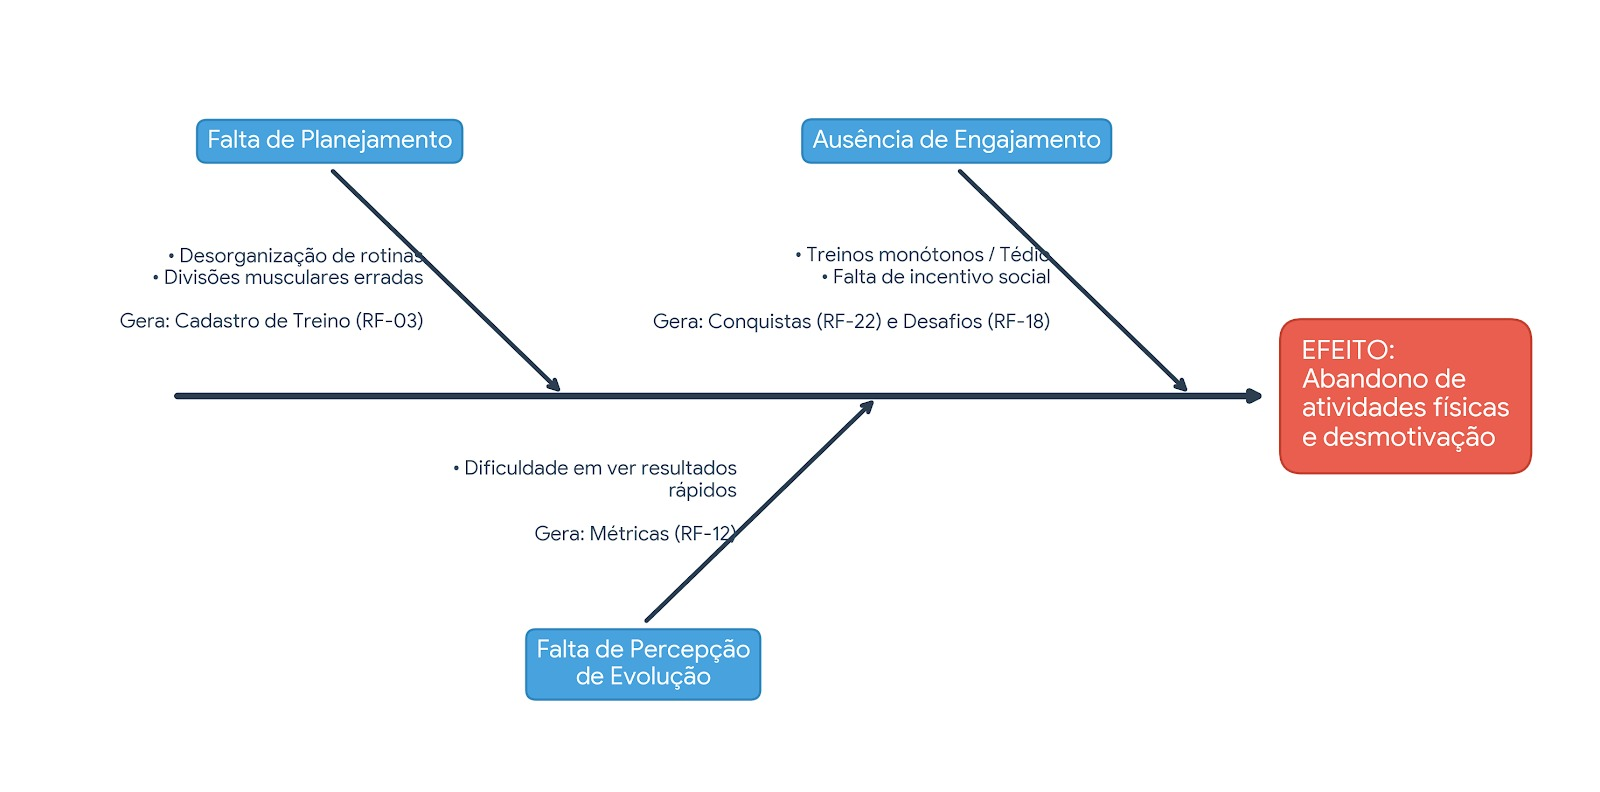
\includegraphics[width=\linewidth,keepaspectratio]{imgs/ishkawa.jpeg}
\par\smallskip
{\fontedez Fonte: elaborado pelos autores (2026), utilizando a técnica de causa e efeito descrita pela ASQ [12].}
\end{figure}
\FloatBarrier

\subsection{PLANEJAMENTO DAS FASES (SPRINTS)}

\noindent\textbf{Abreviações da tabela:} Resp.: responsáveis; \% acum.: percentual acumulado.

O percentual acumulado representa a cobertura funcional planejada, ponderada pelas estimativas preliminares do backlog, e não o progresso real de execução. RF-01 a RF-23 somam 47 unidades estimadas. As Sprints 3 a 9 acrescentam, respectivamente, 7, 6, 8, 6, 7, 7 e 6 unidades: o acumulado arredondado é 15\%, 28\%, 45\%, 57\%, 72\%, 87\% e 100\%. As Sprints 1 e 2 são preparatórias; a Sprint 10 estabiliza as entregas. RF-24 permanece fora do cálculo até receber uma estimativa. O progresso realizado deverá considerar somente funcionalidades concluídas, testadas e aceitas; as estimativas ainda não constituem uma contagem formal de PF.

\begingroup
\small
\setlength{\tabcolsep}{3pt}
\renewcommand{\arraystretch}{1.2}
\begin{longtable}{|>{\raggedright\arraybackslash}p{\dimexpr 0.090\linewidth-2\tabcolsep-1.5\arrayrulewidth\relax}|>{\raggedright\arraybackslash}p{\dimexpr 0.300\linewidth-2\tabcolsep-1.5\arrayrulewidth\relax}|>{\raggedright\arraybackslash}p{\dimexpr 0.170\linewidth-2\tabcolsep-1.5\arrayrulewidth\relax}|>{\raggedright\arraybackslash}p{\dimexpr 0.240\linewidth-2\tabcolsep-1.5\arrayrulewidth\relax}|>{\raggedright\arraybackslash}p{\dimexpr 0.110\linewidth-2\tabcolsep-1.5\arrayrulewidth\relax}|>{\raggedright\arraybackslash}p{\dimexpr 0.090\linewidth-2\tabcolsep-1.5\arrayrulewidth\relax}|}
\caption{Planejamento das sprints}\\
\hline
\textbf{Sprint} & \textbf{Produto (Entrega)} & \textbf{Período} & \textbf{Entregáveis} & \textbf{Resp.} & \textbf{\% acum.} \\ \hline
\endfirsthead
\textbf{Sprint} & \textbf{Produto (Entrega)} & \textbf{Período} & \textbf{Entregáveis} & \textbf{Resp.} & \textbf{\% acum.} \\ \hline
\endhead
1 & Definição do Produto, Documento de Visão, definição do MVP e Planejamento do Projeto. & 22/09/2026 a 27/09/2026 & Documento de visão. & Todos & 0\% \\ \hline
2 & Documento de Arquitetura, base estrutural de projeto e testes. & 28/09/2026 a 04/10/2026 & Documento de Arquitetura, estrutura base e testes, slides das apresentações. & Todos & 0\% \\ \hline
3 & Cadastro de usuário e autenticação com e-mail e senha e treinos (cadastro, listagem, alteração e exclusão de treino). & 05/10/2026 a 11/10/2026 & Backend, Banco de Dados e interfaces base. & Todos & 15\% \\ \hline
4 & Manter exercícios (cadastrar, listar, alterar, excluir e marcar exercício como realizado). Conclusão e validação do MVP com cadastro e login por e-mail e senha, treinos e exercícios. & 12/10/2026 a 18/10/2026 & Testes unitários aprovados e documentação. & Todos & 28\% \\ \hline
5 & Acompanhamento de métricas do usuário, convite de usuário administrador com e-mail. Painel administrativo: visualizar usuários ativos nos últimos 30 dias. & 19/10/2026 a 25/10/2026 & Testes unitários aprovados e documentação. & Todos & 45\% \\ \hline
6 & Painel administrativo: frequência média de treinos, ranking de treinos. & 26/10/2026 a 01/11/2026 & Testes unitários aprovados e documentação. & Todos & 57\% \\ \hline
7 & Painel administrativo: exibir os três exercícios mais realizados pelos usuários. Painel do usuário: submissão de desafios, remoção de desafios. & 02/11/2026 a 08/11/2026 & Testes unitários aprovados e documentação. & Todos & 72\% \\ \hline
8 & Criação do botão de recorde pessoal, sistema de compartilhamento comunitário. & 09/11/2026 a 15/11/2026 & Testes unitários aprovados e documentação. & Todos & 87\% \\ \hline
9 & Inspeções, streak diário, feed de atividades interativo. Integração opcional do login com o Google (RF-24, Could have), conforme a capacidade da equipe. & 16/11/2026 a 22/11/2026 & Testes unitários aprovados e documentação. & Todos & 100\% \\ \hline
10 & Estabilização e entrega: testes, correções de bugs e entrega do produto final. Validação do login com o Google (RF-24, Could have), caso implementado. & 23/11/2026 a 29/11/2026 & Entrega do produto final, documentação final e testes totais. & Todos & 100\% \\ \hline
\end{longtable}
\noindent{\fontedez Fonte: elaborado pelos autores (2026).}
\endgroup

\subsection{MATRIZ DE COMUNICAÇÃO}

\begingroup
\small
\setlength{\tabcolsep}{4pt}
\renewcommand{\arraystretch}{1.2}
\begin{longtable}{|>{\raggedright\arraybackslash}p{\dimexpr 0.250\linewidth-2\tabcolsep-1.5\arrayrulewidth\relax}|>{\raggedright\arraybackslash}p{\dimexpr 0.250\linewidth-2\tabcolsep-1.5\arrayrulewidth\relax}|>{\raggedright\arraybackslash}p{\dimexpr 0.250\linewidth-2\tabcolsep-1.5\arrayrulewidth\relax}|>{\raggedright\arraybackslash}p{\dimexpr 0.250\linewidth-2\tabcolsep-1.5\arrayrulewidth\relax}|}
\caption{Matriz de comunicação}\\
\hline
\textbf{Descrição} & \textbf{Envolvidos} & \textbf{Periodicidade} & \textbf{Produtos Gerados} \\ \hline
\endfirsthead
\textbf{Descrição} & \textbf{Envolvidos} & \textbf{Periodicidade} & \textbf{Produtos Gerados} \\ \hline
\endhead
Acompanhamento das Atividades em Andamento & Toda a equipe do projeto & Semanal & Ata de reunião, relatório de situação do projeto. \\ \hline
Acompanhamento dos Riscos, Compromissos, Ações Pendentes, Indicadores & Toda a equipe do projeto & Semanal & Relatórios focados na resolução de pendências e riscos. \\ \hline
Comunicar situação do projeto & Toda a equipe, Professor e Monitor & Diária & Alinhamentos quanto ao progresso do projeto \\ \hline
\end{longtable}
\noindent{\fontedez Fonte: elaborado pelos autores (2026).}
\endgroup

\subsection{GERENCIAMENTO DE RISCOS}

\begingroup
\small
\setlength{\tabcolsep}{3pt}
\renewcommand{\arraystretch}{1.2}
\begin{longtable}{|>{\raggedright\arraybackslash}p{\dimexpr 0.190\linewidth-2\tabcolsep-1.5\arrayrulewidth\relax}|>{\raggedright\arraybackslash}p{\dimexpr 0.160\linewidth-2\tabcolsep-1.5\arrayrulewidth\relax}|>{\raggedright\arraybackslash}p{\dimexpr 0.120\linewidth-2\tabcolsep-1.5\arrayrulewidth\relax}|>{\raggedright\arraybackslash}p{\dimexpr 0.230\linewidth-2\tabcolsep-1.5\arrayrulewidth\relax}|>{\raggedright\arraybackslash}p{\dimexpr 0.300\linewidth-2\tabcolsep-1.5\arrayrulewidth\relax}|}
\caption{Riscos}\\
\hline
\textbf{Risco} & \textbf{Fase do Projeto} & \textbf{Grau} & \textbf{Mitigação (Prevenção)} & \textbf{Contingência (Reação)} \\ \hline
\endfirsthead
\textbf{Risco} & \textbf{Fase do Projeto} & \textbf{Grau} & \textbf{Mitigação (Prevenção)} & \textbf{Contingência (Reação)} \\ \hline
\endhead
Atraso nas entregas devido ao ciclo curto de 1 semana & Todas as Sprints & Alto & Realizar reuniões de Sprint Planning rigorosas. & Não negociar o aumento da duração da Sprint. As tarefas não concluídas devem ser interrompidas, retornar para o backlog e ser replanejadas para entrega na Sprint imediatamente seguinte. \\ \hline
Abandono/Saída de membro da equipe & Todas as Sprints & Baixo & Fomentar a prática de Pair Programming para evitar que apenas uma pessoa saiba mexer numa parte do código e manter a documentação sempre atualizada. & Redistribuir imediatamente as tarefas críticas pelos restantes membros da equipe e reportar ao P.O. (Monitor Daniel) para reduzir a carga de trabalho (story points) planejada para as Sprints seguintes. \\ \hline
Falha na integração com serviços externos (Autenticação Google) & Sprints 9 e 10 (RF-24, Could have) & Médio & Iniciar os testes de requisição isoladamente via Postman antes de integrar o código ao front-end e back-end. & Manter o cadastro e login com e-mail e senha já disponíveis no MVP (CF-01 e CF-02). Replanejar a integração opcional com o Google (CF-09) sem bloquear as funcionalidades obrigatórias ou comprometer a entrega final. \\ \hline
Desalinhamento com as expectativas do cliente & Sprints de Ponto de Controle & Baixo & Envolver o cliente nas Sprint Reviews, reforçando a cada reunião o cronograma de entregas e deixando claro que o software é entregue em incrementos e ainda se encontra em fase de construção. & Agendar uma reunião extraordinária de alinhamento para relembrar os prazos estritos das Sprints, esclarecendo que qualquer nova exigência não negociada irá para o Backlog para não comprometer o prazo da Sprint atual. \\ \hline
\end{longtable}
\noindent{\fontedez Fonte: elaborado pelos autores (2026).}
\endgroup

\subsection{CRITÉRIOS DE REPLANEJAMENTO}

Os critérios de replanejamento definem os cenários críticos que inviabilizam o cronograma atual. Para o projeto MotivaFit, utilizando a metodologia Scrum, qualquer replanejamento causará o versionamento deste documento. Os critérios adotados são:

\begin{itemize}
\item Abandono da equipe por parte de algum membro, exigindo a readequação dos pontos de esforço da Sprint.
\item Alterações de Escopo: se o cliente ou o Dono do Produto solicitarem mudanças estruturais nos cenários funcionais que ultrapassem a capacidade de entrega semanal da equipe.
\item Atraso crítico em requisitos MUST: caso a equipe atrase e não consiga entregar funcionalidades obrigatórias.
\item Acumulação de Dívida Técnica (Débito Técnico): quando a métrica de débito técnico (falta de refatoração, código não documentado ou ausência de testes) atingir um nível crítico que torne a base de código insustentável, impedindo a equipe de desenvolver e integrar novas funcionalidades com segurança.
\end{itemize}

